\documentclass[
	english,
	fontsize=10pt,
	parskip=half,
	titlepage=true,
	DIV=12
]{scrartcl}

\usepackage[utf8]{inputenc}
\usepackage{babel}
\usepackage[T1]	{fontenc}
\usepackage{lmodern}
\usepackage{microtype}
\usepackage{color}
\usepackage{csquotes}

\usepackage{hyperref}

\newcommand*{\tabcrlf}{\\ \hline}

\usepackage{amsmath}
\usepackage{amssymb}
\usepackage{dsfont}
\usepackage[arrowdel]{physics}
\usepackage{mathtools}
\usepackage{siunitx}

\usepackage{minted}
	\usemintedstyle{friendly}

\newcommand*{\inPy}[1]{\mintinline{python3}{#1}}
\newcommand*{\ie}{i.\,e. }
\newcommand*{\eg}{e.\,g. }

\begin{document}

\part*{Python Problems 04, Summer 2021}
The following problems are very physics inspired and very maths-y. This is due to the fact that the module SciPy was written specifically with the intent of solving mathematical/physical problems. I've done my best to find a good balance between \emph{interesting problems} and \emph{manageable for an average student}. However, to do so I had to assume you have a good grasp of the mathematical concepts involved, \ie you're enrolled in some science degree. If you have problems understanding the problems, rest assured that next week's problem set will be more about \emph{generic programming skills} again.

Also, don't be intimidated by the length of this sheet. The entire problem set can be solved in less than 250 lines of code ;)

\section{Sun's Surface Temperature}
On GRIPS you will find the file \texttt{astmg173.csv} which contains our sun's emission spectrum as measured from different observatories\footnote{The original data can be found on \url{https://www.nrel.gov/grid/solar-resource/spectra-am1.5.html}}. The first column is the \emph{wavelength} and the second column is the \emph{irradiance} (radiant power per unit area). You can ignore the other columns.

The sun's spectrum is primarily given by its temperature. Planck's law states the following relation between irradiance $B$, emitted wavelength $\lambda$ and temperature $T$:

\[ B(\lambda ,T)={\frac {2hc^{2}}{\lambda ^{5}}}{\frac {1}{e^{\frac {hc}{\lambda k_{\mathrm {B} }T}}-1}} \]

Use this to determine the sun's surface temperature by fitting the above function to the spectral data in the file. Plot the spectral data and the fit. You can use the following implementation of Planck's law which already accounts for unit conversion:
\begin{minted}{python3}
def planck(wavelength, T) :
    # see https://en.wikipedia.org/wiki/Planck%27s_law
    wl = 1e-9 * wavelength      # input is in nanometers; we need SI units
    
    return  (2 * h * c**2) / (wl**5) * \
            1E-13 / (np.exp( (h * c) / (wl * kB * T) ) - 1)
\end{minted}

\emph{Background Information}:\\
The literature value for the sun's surface temperature is \SI{5778}{K} and was found exactly as we did by fitting spectral data against Planck's law. However, earth's atmosphere absorbs a significant portion of the sun's light. Further, there's axial tilt and other subtleties to be factored in. Don't worry if your result is several hundred Kelvin off, but do make sure your result is at least in the \SI{5000}{K} regime.

\section{Fourier Transform of an Image}
The function \texttt{scipy.misc.ascent} returns a NumPy 2D array of \texttt{np.int64} values that can be interpreted as an greyscale image. Use MatPlotLib's \texttt{imshow} to display the image\footnote{You'll find example code for that on \url{https://docs.scipy.org/doc/scipy/reference/generated/scipy.misc.ascent.html}}.

Now compute the 2D Fourier Transform of that image. Use the FFT module of SciPy for that. You can look up the functions under \inPy{https://docs.scipy.org/doc/scipy/reference/fft.html}. The Transform of an image is a 2D array of complex numbers. You can compute the logarithm of the absolute value of each point (\texttt{np.log(np.abs(transform)}) and plot that array as an image, too. Can you explain what the bright and dark spots mean?

Implement a \emph{High Pass Filter}, \ie set the pixels in the transform corresponding to low frequencies to zero. Compute the inverse Fourier Transform and plot it. Play around with these tools to get a feeling for them.

\emph{Background Information}:\\
The (Fast) Fourier Transform is the core of JPEG compression: Instead of storing the individual pixel brightnesses, first the FT is computed. Then, the algorithm \enquote{throws out} the modes with the lowest contributions, effectively reducing the amount of data that needs to be stored. There's some more maths involved, but the basic idea is \enquote{just} that. Do you now understand why JPEG is \emph{lossy} compression and where JPEG artefacts come from?

\section{Orbit}
Numerically, find the trajectory of an object in a $^{1}/_{r}$ potential in 2D space! To do so, follow these steps:

Understand the following differential equation:
\[ \ddot{\vec{x}} = -\frac{1}{r} \frac{\vec{x}}{\abs{\vec{x}}} \]

So we have a \emph{second order} differential equation in \emph{two components} (we are in 2D space). So in total we need to create a system of \emph{four first order differential equations}. Follow the scheme shown in the lecture and create a function that implements this system of equations.

Now define the initial conditions. Understand that we need \emph{four} givens for our system of four first order differential equations. Setting 
$\vec{x}(0) = \begin{pmatrix}
	0 \\ 1
\end{pmatrix}$
and
$\dot{\vec{x}}(0) = \begin{pmatrix}
	0.4 \\ 0
\end{pmatrix}$
should give a nice orbit, but you are free to toy around as you like.

Set up the times at which the trajectory should be evaluated. Doing this with for 1000 times between 0 and 100 should give nice results for the above mentioned initial conditions, but feel free to toy around.

Now plut all these data into SciPy's solver for ODEs and plot the result. Below you see an example output. Red is the origin, \ie the \enquote{source} of the potential (think of a star around which our object orbits). The blue dot is the initial position of the object, and the curve is its trajectory around the star.
\begin{center}
	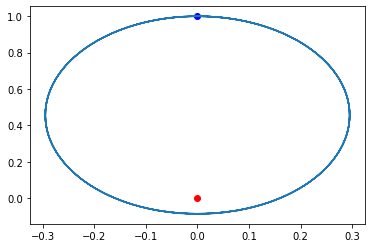
\includegraphics[width=.4\linewidth]{./orbit-example}
\end{center}

What happens when you increase the maximum time? What happens if you decrease the number of time steps? What happens if you increase both, maximum time and time steps?

\section{Heat Equation}
Now let's go wild and use our understanding from the last exercise to solve a \emph{PDE}! Specifically, we want to tackle the heat equation:
\[ \pdv{T}{t} = \alpha \laplacian T \]

That is, we have a time dependent scalar field $T(\vec{x}, t)$: the temperature $T$ at some location $\vec{x}$ and some time $t$. We will do so on a \emph{discrete grid}, \ie we will regard a matrix-like object $T_{ij}(t_k)$, evaluated at \emph{discrete} times $t_k$ and in \emph{discrete} locations $\vec{x}_{ij}$:
\begin{align*}
	T_{ij}(t_k) &= T(\vec{x}_{ij}, t_k) \\
	\vec{x}_{ij} &= i \Delta x \vec{\text{e}}_1  + j \Delta x \vec{\text{e}}_2 \\
	t_k &= k \Delta t
\end{align*}
So our grid has a \emph{spatial resolution} of $\Delta x$ and a \emph{temporal resolution} of $\Delta t$. In the end, we will deal with a \emph{tensor of third order}, $T_{kij}$

\subsection{Derivatives in the Finite Difference Scheme}
First, we need a means to evaluate $\laplacian T$. For this, let's go back and see how a \emph{first order derivative} of a \emph{one dimensional} function is defined and what that means in a discrete grid:
\[ \dv{x} f(x) = \lim_{h \to 0} \frac{f(x + h) - f(x)}{h} \]

On a discrete grid, we cannot go $h \to 0$; the smallest difference possible is $h = \Delta x$. With this, the differential quotient becomes:
\begin{align*}
	f_i &= f(x_i) \\
	\Delta f_i &= \frac{f_{i + 1} - f_i}{\Delta x}
\end{align*}

For reasons of numerical stability, the \emph{symmetric form} is preferred:
\begin{align*}
	\Delta f_{i} &= \frac{f_{i + 1} - f_{i - 1}}{2\Delta x}
\end{align*}

Likewise, for a 2D grid we can approximate the derivative as:
\begin{align*}
	f_{ij} &= f(x_{ij}) \\
	\Delta f^{(x)}_{ij} 
&=
	\frac{f_{i + 1, j} - f_{ij} + f_{i + 1, j} - f_{ij}}{\Delta x} \\
&=
	\frac{f_{i + 1, j} + f_{i + 1, j} - 2 f_{ij}}{\Delta x}
\\
	\Delta f^{(y)}_{ij} 
&=
	\frac{f_{i, j + 1} + f_{i, j + 1} - 2 f_{ij}}{\Delta x}
\end{align*}


Likewise, an expression for the second derivative can be found.

This now could be done by means of two nested \inPy{for} loops; for reasons of efficiency, however, we want to use a \emph{vectorized} approach: We'll do a \emph{convolution with a matrix}.

For two matrices\footnote{I'll assume them to be real valued; however, this works for any field $\mathbb{K}$ you fancy.} $A, B$, the convolution $A \ast B$, is defined as follows:\\
Let $A \in \mathbb{R}^{n \times m}$ and $B \in \mathbb{R}^{s \times t}$
\begin{align*}
	(A \ast B)_{\substack{
		i = 1 ... n-r\\
		j = 1 ... m-s
	}}
&=
	\sum_{k = 1}^{r}
	\sum_{l = 1}^{t}
		A_{i-k+1, j-l+1} B_{kl}
\end{align*}

With this formalism, we can express the Laplacian as a matrix:
\[ 
	\laplacian_{\Delta x} 
= 
	\frac{1}{\Delta x^2}
	\begin{pmatrix}
		 0 &  1 &  0 \\
		 1 & -4 &  1 \\
		 0 &  1 &  0
	\end{pmatrix}
\]
and the Laplacian of our scalar field by a convolution:
\[ (\laplacian T)_{ij} = (T \ast \laplacian_{\Delta x})_{ij} \]

The convolution can be computed by means of \texttt{scipy.signal.convolve}. Read up on how to use that command on \url{https://docs.scipy.org/doc/scipy/reference/generated/scipy.signal.convolve.html}. Then try to use it on this code:
\begin{minted}{python3}
laplacian_matrix = deltaX**2 * np.array(
        [[ 0,  1,  0],
         [ 1, -4,  1],
         [ 0,  1,  0]])

quadraticInX = np.array([[x**2 for x in range(5)] for row in range(5)])

print(quadraticInX)
nablaSquaredQIX = # your code here
print(nablaSquaredQIX)
\end{minted}

The output should look like this:
\begin{minted}{text}
[[ 0  1  4  9 16]
 [ 0  1  4  9 16]
 [ 0  1  4  9 16]
 [ 0  1  4  9 16]
 [ 0  1  4  9 16]]
[[  1   1  -2  -7 -39]
 [  1   2   2   2 -23]
 [  1   2   2   2 -23]
 [  1   2   2   2 -23]
 [  1   1  -2  -7 -39]]
\end{minted}

Why are the values in the top/bottom row and left/right column of the matrix garbage?

\emph{Hint}:\\
Have a look at the optional parameter \texttt{mode} in the documentation.

\subsection{Vectorized Time Derivative}
Now that we can compute $\laplacian T$, we can attack solving the PDE. We recall that
\[ \pdv{T}{t} = \alpha \laplacian T \]
\ie we have a \emph{first order} differential equation -- which makes it much easier in the following. In theory we could simply \inPy{return resultOfConvolution} and be done with. Unfortunately, using \texttt{scipy.integrate.odeint} requires us to use a 1D vector for all components of our system, but \texttt{T} has to be at least \emph{2}-dimensional to represent our grid.

To remedy this, we can use a trick: by means of \texttt{T.reshape} we can make T have any dimension we want to (provided we don't add or remove numbers, which we don't want to). That is, we can make a vector out of a \texttt{T} matrix when we hand it over to the \texttt{odeint} code and we can make a matrix out of a vector when we hand it over to \texttt{scipy.signal.convolve}.

With these ideas, complete the following blueprint for the time derivative function:
\begin{minted}{python3}
def heatODE(T, t, alpha, Nx, Ny) :
    # dT/dt = alpha laplacian T

    # your code here
    # dT = ...
    # your code here
    
    return dT
\end{minted}

\subsection{Implementing Boundary Conditions}
You may be aware of the fact that for a PDE we need an extended set of boundary conditions. Here, we'll use \emph{Dirichlet boundary conditions}. That means, we'll fix the temperature field at $t = 0$ and further also require the temperature at the boundaries to be constant. In other (more maths-y) words, we want:
\begin{align*}
	T(\vec{x}, t = 0) &= T_0(\vec{x}) 
	&&
	\forall \vec{x} \in \Omega
\\
	\pdv{T}{t}(\vec{x}) &= 0
	&&
	\forall \vec{x} \in \partial \Omega, \forall t \in \mathbb{R}_{0}^{+}
\end{align*}

In particular, let's make it so that the boundary of our grid is kept at fixed temperatures. This corresponds to a sheet of some material heated from one side and cooled from the others. We'll define:
\begin{align*}
	T_0(\vec{x})
&=
	\begin{cases}
		10 & \text{if } x_1 = 0 \\
		 0 & \text{otherwise}
	\end{cases}
\end{align*}

Now, define a variable \texttt{T0} that obeys this definition. At first, keep the system dimensions small -- say a $10 \times 10$ grid (otherwise, the next steps will take a long time). You can later change the grid size to any value you like. Also, alter your function \texttt{heatODE} such that it obeys 
$\pdv{T}{t}(\vec{x}) = 0 \forall \vec{x} \in \partial \Omega, \forall t \in \mathbb{R}_{0}^{+}$.

\subsection{Putting it all Together}
Define the NumPy-Array \texttt{t} for 100 times between 0 and 100. Make it so that your 2D array \texttt{T0} is converted into a 1D vector. Pass it all to \texttt{scipy.integrate.odeint}. 

If everything went correctly, you should be able to \enquote{harvest} the following plots:
\begin{center}
	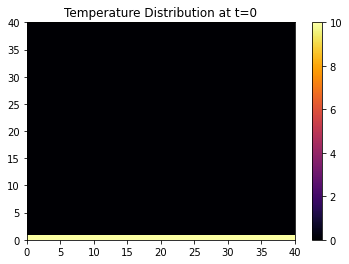
\includegraphics[width=.3\linewidth]{./TDist-0}
	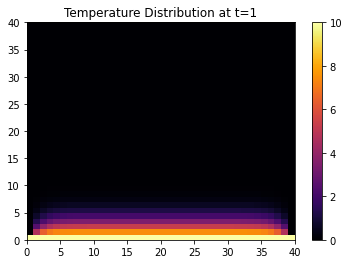
\includegraphics[width=.3\linewidth]{./TDist-1}
	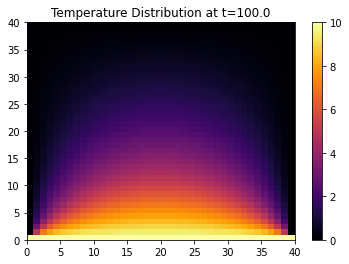
\includegraphics[width=.3\linewidth]{./TDist-100}
\end{center}
\end{document}
